% Left: a monotone path from (0,0) to (4,3) is a word in E and N. Right: the reflection of a path
% to (4,4) that touches the line y=x+1, giving a path to (3,5). Generated by figs_t0c01.py.
\begin{tikzpicture}[scale=0.55]
\begin{scope}
\draw[black!25] (0,0) grid (4,3);
\draw[MidnightBlue,very thick] (0,0) -- (1,0) -- (1,1) -- (2,1) -- (3,1) -- (3,2) -- (4,2) -- (4,3);
\fill[MidnightBlue] (0,0) circle (3pt); \fill[MidnightBlue] (4,3) circle (3pt);
\node[font=\small,anchor=north] at (2,-0.3) {$\mathsf{ENEENEN}$: $\binom73=35$ paths to $(4,3)$};
\end{scope}
\begin{scope}[xshift=7.5cm]
\draw[black!25] (0,0) grid (5,5);
\draw[BrickRed!70,dashed,thick] (-0.3,0.7) -- (4.3,5.3) node[anchor=south west,font=\scriptsize,BrickRed] {$y=x+1$};
\draw[black!50,thin] (0,0) -- (4.6,4.6);
\draw[MidnightBlue,very thick] (0,0) -- (1,0) -- (1,1) -- (1,2);
\draw[MidnightBlue,very thick,densely dotted] (1,2) -- (1,3) -- (2,3) -- (3,3) -- (4,3) -- (4,4);
\draw[BrickRed,very thick] (1,2) -- (2,2) -- (2,3) -- (2,4) -- (2,5) -- (3,5);
\fill[BrickRed] (1,2) circle (3.5pt);
\fill[MidnightBlue] (4,4) circle (3pt) node[anchor=west,font=\scriptsize] {$(4,4)$};
\fill[BrickRed] (3,5) circle (3pt) node[anchor=south,font=\scriptsize] {$(3,5)$};
\node[font=\small,anchor=north,text width=5.4cm,align=center] at (2.5,-0.3) {a path that crosses the diagonal is reflected after its first point on $y=x+1$};
\end{scope}
\end{tikzpicture}
